\documentclass[tikz, border=10pt]{standalone}
\usepackage{tikz}
\usetikzlibrary{calc}

\begin{document}
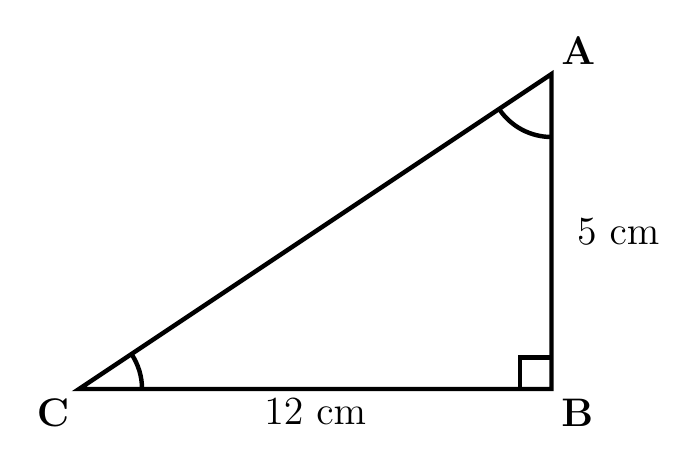
\begin{tikzpicture}

% Define vertices
\coordinate (A) at (6, 4);
\coordinate (B) at (6, 0);
\coordinate (C) at (0, 0);

% Draw the triangle
\draw[ultra thick] (A) -- (B) -- (C) -- cycle;

% Right angle mark at B
\def\sq{0.4}
\draw[ultra thick] (B) ++(-\sq, 0) -- ++(0, \sq) -- ++(\sq, 0);

% Angle arc at A
\pgfmathsetmacro{\angleCA}{atan2(-4, -6)}
\draw[ultra thick] ($(A)+(270:0.8)$) arc (270:213.7:0.8);

% Angle arc at C
\pgfmathsetmacro{\angleAC}{atan2(4, 6)}
\draw[ultra thick] ($(C)+(0:0.8)$) arc (0:\angleAC:0.8);

% Labels for vertices
\node[above right] at (A) {\textbf{\Large A}};
\node[below right] at (B) {\textbf{\Large B}};
\node[below left] at (C) {\textbf{\Large C}};

% Dimension labels in Bangla
% Right side: AB = 5 cm
\node[right, font=\Large] at ($(A)!0.5!(B)+(0.2,0)$) {5 cm};

% Bottom side: CB = 12 cm
\node[below, font=\Large] at ($(C)!0.5!(B)$) {12 cm};

\end{tikzpicture}
\end{document}